\mychapter{Características de um Rede Multi VANTs}
\label{Cap:Requisitos}

\begin{comment}
A utilização de redes multi VANTs se deu pela sua eficiência em tempo e custo em relação a redes de um único VANT na realização de missões dos mais variados tipos. \cite{gupta2015survey} descreve em seu trabalho as características únicas que garantem as redes multi VANTs essa vantagem competitiva.

Em \emph{Survey of Important Issues in UAV Communication Networks}, Gupta compara as características das redes de comunicação multi VANTs com redes MANET e VANET que, respectivamente, são redes para comunicação \emph{mobile} e comunicação veicular. Essa comparação é feita devido a similaridades entre as mesmas, no entanto, conclui-se que os trabalhos nessas duas áreas não atendem por completo as necessidades especificas de uma rede multi VANTs.

Por exemplo, a complexidade do modelo de mobilidade dos nós em uma rede multi VANTs não se compara ao das redes VANETs ou MANETs. Um nó em uma rede multi VANTs pode se mover de forma randômica ou ordenada, dependendo da natureza da missão a ser executada, e esse movimento pode ocorrer nas três dimensões, enquanto os nós de uma rede VANETs ou MANETs irão se mover de forma mais previsível e realizarão o movimento em apenas duas dimensões, ao longo de um rodovia como é o caso da rede VANETs. Dessa forma, as mudanças em topologia de uma rede multi VANTs serão mais frequentes.

Além da questão da mobilidade dos nós, outra característica das rede multi VANTs que influencia nas frequentes mudanças de topologia da rede seria o acesso limitado a energia e o curto tempo de voo de um VANT, algo em torno de trinta minutos com uma carga. Nós serão desligados da rede devido a baixos níveis de bateria ou mal funcionamento e outros serão adicionados a rede para substituir os nós perdidos, quando necessário.

Por outro lado, como são formadas por vários nós, as redes multi VANTs são mais confiáveis quando comparadas com redes compostas por um único VANT. Em cenário onde um dos nós da rede perde conexão, a rede pode se reorganizar e garantir a sobrevivência da mesma. No entanto, essa reorganização topológica se traduz em um consumo extra de energia na rede por completo, dessa forma, reafirmando a importância de uma rede implementada de forma otimizada quanto ao consumo energético. 

Portanto, a rede multi VANTs possuem características especificas que a diferencia de outra redes tais quais a complexidade da mobilidade dos nós, o poder de reorganização da rede para garantir a sobrevivência e escalabilidade da mesma e, por consequência disso tudo, a necessidade de otimização do consumo energético para garantir maior tempo de operação do sistema como um todo.
\end{comment}

As redes multi VANTs são uma evolução das redes formadas por apenas um VANT e a base de controle, onde toda a troca de informações é realizada atraves de um \emph{link} entre as duas partes do sistema e caso esse \emph{link} fosse quebrado por algum motivo toda a rede era desfeita. A rede multi VANTs, então, com intuito de aumentar o alcance e a confiabilidade da rede através da adição de novos nós.

\cite{gupta2015survey} apresenta algumas das característica de uma rede multi VANTs comparando-as a solução de um único VANT, sendo elas:
\begin{itemize}
\item Escalabilidade
\item Capacidade de Sobrevivência
\item Velocidade da Missão
\item Complexidade do Controle
\item Economia de Energia
\end{itemize} 

\section{Escalabilidade}

Por definição uma rede multi VANTs é uma versão escalada da solução composta por VANT mais base de controle. Dessa forma, a adição de nós se torna uma operação comum a uma rede multi VANTs tornando-o uma solução escalável que pode variar o tamanho e, consequentemente, o alcance da rede dada as necessidades especificas da missão.

\section{Capacidade de Sobrevivência}

Como mencionado anteriormente, na solução formada por VANT mais base de controle, a rede é composta por apenas um \emph{link} e caso esse seja quebrado a comunicação entre os nós dessa rede será perdida. No entanto, dado que uma rede multi VANTs será formada múltiplos nós e \emph{links}, em caso da perda de um nó a rede pode se reorganizar e garantir a sobrevivência da rede como um todo. 

Por exemplo, em uma rede composta por quatro nós em topologia \emph{mesh} como mostra a fig. \ref{fig:perdaNo}, no caso de falha do nó B, a comunicação entre os nós entre os nós A e D poderá ser feita através do nó C, garantindo assim a sobrevivência da rede. 

\begin{figure} 
\center
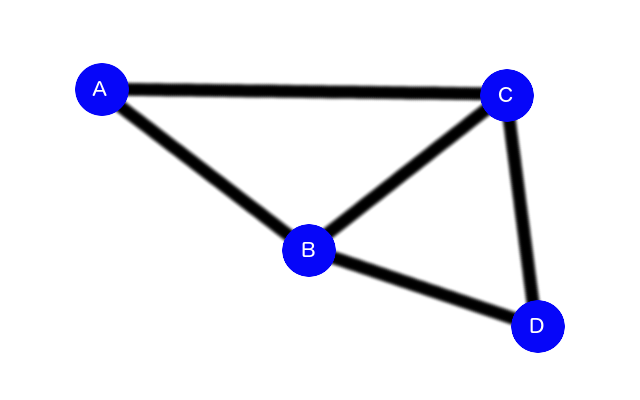
\includegraphics[width=0.7\textwidth]{perdaNo.png}
\caption{Esquema rede multi VANTs com 4 nós.} 
\label{fig:perdaNo}
\end{figure} 

\section{Velocidade da Missão}

A velocidade de realização de uma determinada missão será proporcional ao tamanho da rede multi VANT, quanto maior a quantidade de VANTs em uma determinada rede a ser utilizada para executar uma missão de varredura de área, menor será o tempo da missão. Por outro lado, a adição de um nó a uma rede resultará no aumento do custo da missão. Dessa forma, é importante analisar os benefícios do aumento de uma rede multi VANTs do ponto de vista financeiro. 

\section{Complexidade do Controle}

A complexidade do controle de uma rede composta por apenas um VANT e uma base de controle é baixa quando comparado ao cenário de uma rede multi VANTs. Quanto maior a quantidade de nós em uma rede maior será o custo computacional para controlar os nós e determinar os caminhos para realização da comunicação entre eles.

Outro ponto que aumente ainda mais essa complexidade é a frequente mudança de topologia da rede, seja causada pela movimentação rápida dos nós, que se dá nas três dimensões, ou pela perda de nós devido a problemas de funcionamento ou fim da carga da bateria de alimenta o VANT.

\section{Economia de Energia}

Como VANTs possuem fonte de alimentação limitada, é importante garantir que rede funcione da forma mais eficiente possível quanto ao consumo de energia, de tal forma que os nós possam permanecer ativos na rede pelo máximo de tempo possível. Caso a rede de comunicação consuma muita energia dos VANTs, será necessário a substituição de nós durante a execução de uma missão o que, consequentemente, aumentará o tempo necessário para a realização da mesma.\\

As características discutidas nessa sessão servirão de base para produção do protocolo de testes e, por fim, desenvolvimento da arquitetura de rede a ser implementada futuramente. 